\chapter{Advanced Functions}\label{appendix:advutil}

There are a few advanced functions that once can use in a \glsfirst{SB}.

%============================================================================
\section{General Functions}

%****************************************************

\subsection{GetValue()}

The {\bfseries{\textcolor{pythonKeywords}{GetValue}}()} function can be used
to retrieve any parameter or sampler value within the \glsfirst{MC} system.

\begin{description}[itemsep=1pt]
\item[{\bf SYNTAX}:]
value = {\bfseries{\textcolor{pythonKeywords}{GetValue}}(}
\sq{manager}, \sq{parameter,parameter\_field}
{\bf)}

\begin{description}[leftmargin=*]
\item[value] A string. If you need the return value to be another data type
such as an integer or float, plase consult your favorite Python manual to find
out how to use conversion operators.
\item[manager] A manager in the \gls{MC} system such as \sq{scanCoordinator}
\item[parameter] The name of the parameter or sampler value to retrieve.
\item[parameter\_field] The name of the parameter or sampler field value to retrieve.
\end{description}
\item[{\bf USAGE}:] Please consult with your scientific contact person.
\end{description}

\lstinputlisting[language=PythonAstrid,
backgroundcolor=\color{sbBackground},
caption={[GetValue() example.]
GetValue() example.},
label={lst:getvalue}]
{getvalue.py}


%****************************************************************************
\newpage

\subsection{SetValues()}

The {\bfseries{\textcolor{pythonKeywords}{SetValues}}()} function can be used
to directly set any of the parameters within the \gls{MC} system.  As a result,
it is used to support complex configurations and expert observations. Please
note that {\bfseries{\textcolor{pythonKeywords}{SetValues}}()} does not always
issue a \dq{prepare} on the \gls{MC} Manager containing the parameter. If 
you wish to do a \dq{prepare}, you can also use
{\bfseries{\textcolor{pythonKeywords}{SetValues}}()} to do that as well. 

\begin{description}[itemsep=1pt]
\item[{\bf SYNTAX}:]
{\bfseries{\textcolor{pythonKeywords}{SetValues}}(}
\sq{manager}, {\bf\{}\sq{parameter,parameter\_field: value}{\bf\}}
{\bf)}

\begin{description}[leftmargin=*]
\item[manager] The manager containing the parameter in the \gls{MC} system.
\item[parameter] The name of the parameter.
\item[parameter\_field] The name of the parameter field.
\item[value] The actual value to set. Data types depend on the parameter.
\end{description}
\item[{\bf USAGE}:] Please consult with your scientific contact person.
\end{description}

\lstinputlisting[language=PythonAstrid,
backgroundcolor=\color{sbBackground},
caption={[SetValues() example.]
SetValues() example.},
label={lst:setvalues}]
{setvalues.py}

%****************************************************************************
\subsection{DefineScan()}

If you have written your own scan type using the Python language, 
the {\bfseries{\textcolor{pythonKeywords}{DefineScan}}()} function is used to
load your new scan type into the current \gls{SB}. Once loaded, it can be
referred to by name, just like any other scan type.

\begin{description}[itemsep=1pt]
\item[{\bf SYNTAX}:]
{\bfseries{\textcolor{pythonKeywords}{DefineScan}}(}
scanName , filepath
{\bf)}

\begin{description}[leftmargin=*]
\item[scanName] A string specifying a name for the scan.
\item[filepath] A string specifying the full filepath to the scan.
\end{description}
\item[{\bf USAGE}:] The following example defines and then executes a scan used
                    primarily with \gls{MUSTANG} observations.
\end{description}

\lstinputlisting[language=PythonAstrid,
backgroundcolor=\color{sbBackground},
caption={[DefineScan() example.]
DefineScan() example.},
label={lst:definescan}]
{definescan.py}

%****************************************************************************
\subsection{GetCurrentLocation()}

Given a coordinate mode,
{\bfseries{\textcolor{pythonKeywords}{GetCurrentLocation}}()} returns a
Location object 

\begin{description}[itemsep=1pt]
\item[{\bf SYNTAX}:]
value = {\bfseries{\textcolor{pythonKeywords}{GetCurrentLocation}}(}
coordinateMode
{\bf)}

\begin{description}[leftmargin=*]
\item[value] A Location object (see \S~\ref{sec:location_objects}) containing the
coordinates of the currently selected receiver beam's position on the sky (as
selected in the most recent scan type).
\item[coordinateMode] A string specifying the coordinate mode of the Location
object in the return value.  Available coordinate modes are \sq{J2000},
\sq{B1950}, \sq{RaDecOfDate}, \sq{HaDec}, \sq{ApparentRaDec}, \sq{Galactic},
\sq{AzEl}, and \sq{Encoder}.
\end{description}
\item[{\bf USAGE}:] The following example prints the current coordinates in
azimuth and elevation.  Note that GetH() and GetV() return float values for
the major and minor axis coordinates of Location and Offset objects.
\end{description}

\lstinputlisting[language=PythonAstrid,
backgroundcolor=\color{sbBackground},
caption={[GetCurrentLocation() example.]
GetCurrentLocation() example.},
label={lst:getcurrentlocation}]
{getcurrentlocation.py}


%****************************************************************************

\subsection{SetSourceVelocity()}

The {\bfseries{\textcolor{pythonKeywords}{SetSourceVelocity}}()} function sets
the \gls{LOone} source velocity directly, in units of km/s.

\begin{description}[itemsep=1pt]
\item[{\bf SYNTAX}:]
value = {\bfseries{\textcolor{pythonKeywords}{SetSourceVelocity}}(}
velocity
{\bf)}
\begin{description}[leftmargin=*]
\item[velocity] The source velocity in km/s.
\end{description}
\item[{\bf USAGE}:] If you include the velocities in your catalog
(see \S~ref{sec:catalogs}) then you do not need to use this function.
\end{description}

\lstinputlisting[language=PythonAstrid,
backgroundcolor=\color{sbBackground},
caption={[SetSourceVelocity() example.]
SetSourceVelocity() example.},
label={lst:setsourcevelocity}]
{setsourcevelocity.py}

\newpage

%============================================================================
\section{Specialty Scan Types}\label{appendix:scantype}

%herez

%-----------------------------------------------------------------------------
\subsection{Spider}

{\bfseries{\textcolor{pythonKeywords}{Spider}}()} executes the specified number
of slices of duration {\bf scanDuration} through the specified location. Each slice
is of length 2*{\bf startOffset}. The argument startOffset also specifies the angle
of the initial slice. The user may specify unidirectional or bidirectional
subscans of length {\bf calDuration} and when to run calibration subscans relative
to each slice, i.e., at \sq{begin}, \sq{end}, or \sq{both}.

\begin{description}
\item[{\bf SYNTAX}:]\ \\
{\bfseries{\textcolor{pythonKeywords}{Spider}}(}
location, startOffset, scanDuration, slices, beamName, unidirectional, cals, calDuration
{\bf)}
\item[location] A Catalog source name or Location object. It specifies the 
source which is to be tracked.
\item[startOffset] An Offset object. It specifies the 1/2 length of the 
subscans and the angle from location of the initial subscan. For example, If 
startOffset = {\bfseries{\textcolor{pythonKeywords}{Offset}}(}
\sq{AzEl}, \sq{00:40:00},\sq{00:00:00},cosv=True
{\bf)}
then the first leg of the scan would start at +40\arcminute\ in azimuth 
(from the location) and would complete at -40\arcminute\ in AZ.
If instead you used
startOffset = {\bfseries{\textcolor{pythonKeywords}{Offset}}(}
\sq{AzEl}, \sq{00:40:00},\sq{00:40:00},cosv=True{\bf)}
the first leg would start at AZ=+40\arcminute, EL=+40\arcminute, and would 
go to the opposite (AZ=-40\arcminute, EL=-40\arcminute).
\item[scanDuration] A float. It specifies the length of the subscans in 
seconds.
\item[slices] An integer. It specifies the number of subscans through 
location. The default is 4 (making a spider shape -- i.e eight legs).
\item[beamName] A string. It specifies the receiver beam to use for the 
scan. beamName can be \sq{C}, \sq{1}, \sq{2}, \sq{3}, \sq{4} or any valid
combination for the receiver you are using such as \sq{MR12}. The default
is \sq{1}.
\item[unidirectional] A Boolean. It specifies whether each slice is scanned 
once in one direction or twice in both directions. The default is True (one 
direction).
\item[cals] A string. It specifies the order of calibration subscans, i.e., 
at the beginning of the slice subscan (\sq{begin}), at the end of the slice 
subscan (\sq{end}), or both (\sq{both}). The default is \sq{both}.
\item[calDuration] A float. It specifies the length of the calibration 
subscans in seconds. The default is 10.0.
\item[{\bf USAGE}:]\ \\
Script~\ref{lst:spider} generates subscans through 3C~286 starting the first
leg 40\arcminute\ from the source's \dq{right}.  A plot showing the actual
trajectory on the sky when the script was executed is shown in figure
\ref{fig:spider}.  Black crosses mark timestamps of data sampled
along the red trajectory.
\end{description}

\lstinputlisting[language=PythonAstrid,
backgroundcolor=\color{sbBackground},
caption={[Spider() example.]
Spider() example.},
label={lst:spider}]
{spider.py}

\newpage
\noindent\begin{minipage}[t]{0.485\linewidth}
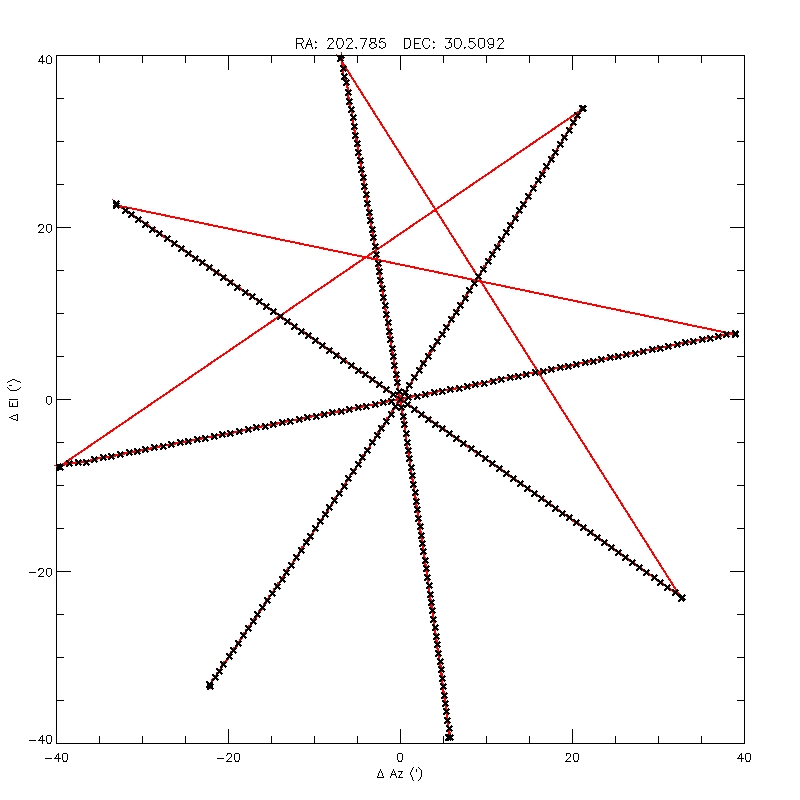
\includegraphics [width=\linewidth] {spider.jpg}
\captionof{figure}[Spider() GBT Antenna Trajectory]
{The actual Spider() trajectory (red) on the sky generated by executing script~\ref{lst:spider}.
Crosses mark timestamps of sampled data. (sampling period is set via {\bf tint} in the
configuration).\label{fig:spider}}
\end{minipage}
\hfill
\begin{minipage}[t]{0.485\linewidth}
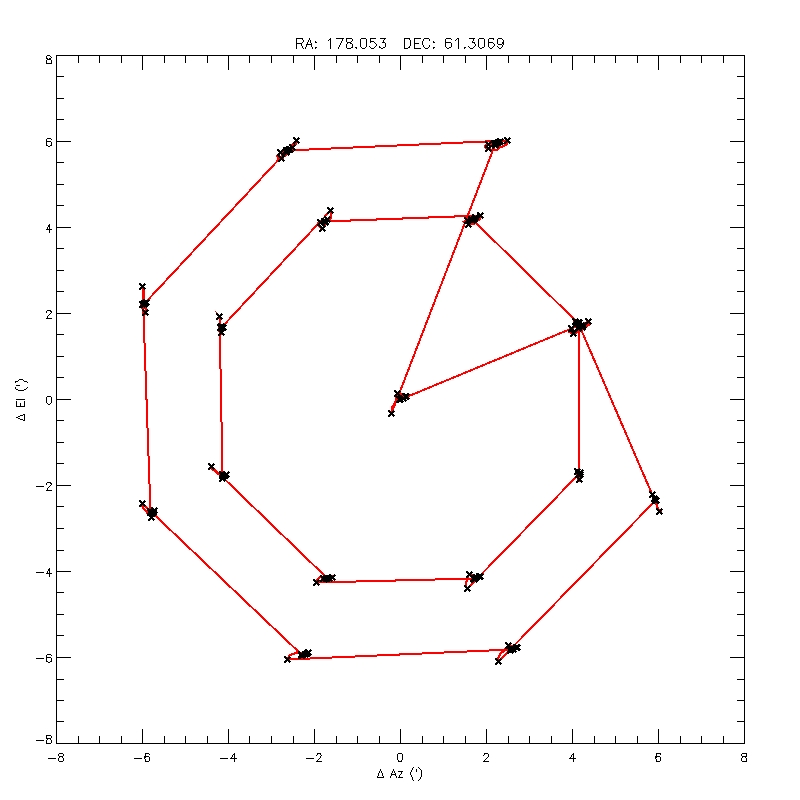
\includegraphics [width=\linewidth] {z17.jpg}
\captionof{figure}[Z17() GBT Antenna Trajectory]
{The actual Z17() tracjectory (red) on the sky generated by executing script~\ref{lst:z17}.
Crosses mark timestamps of sampled data at each point.\label{fig:z17}}
\end{minipage}


\subsection{Z17}

{\bfseries{\textcolor{pythonKeywords}{Z17}}()} executes two circles of
point subscans around location at 45$^\circ$ intervals. The first circle
with a radius of {\bf startOffset} and the second circle at a radius
of $\sqrt{2}{\cdot}${\bf startOffset}. The initial subscan is at the 
angle specified by the {\bf startOffset}. After circling twice, the
procedure executes a subscan on location. The entire set of 17 subscans each of 
length {\bf scanDuration}, is sandwiched between two cal subscans of lengths 
{\bf calDuration} which consist of equal parts calibration noise signal on
and off.

\begin{description}
\item[{\bf SYNTAX}:]\ \\
{\bfseries{\textcolor{pythonKeywords}{Z17}}(}
location, startOffset, scanDuration, beamName, calDuration
{\bf)}
\item[location] A Catalog source name or Location object. It specifies the 
source which is to be tracked.
\item[startOffset] An Offset object. It specifies the angle from location of 
the initial subscan as well as the radius of the inner circle.
\item[scanDuration] A float. It specifies the length of the subscans in 
seconds.
\item[beamName] A string. It specifies the receiver beam to use for the 
scan. beamName can be \sq{C}, \sq{1}, \sq{2}, \sq{3}, \sq{4} or any valid
combination for the receiver you are using such as \sq{MR12}. The is \sq{1}.
\item[calDuration] A float. It specifies the length of the calibration 
subscans in seconds. The default is 10.0.
\item[{\bf USAGE}:] Script~\ref{lst:z17} generates subscan points
around G135.1+54.4 starting the first circle at the source's \dq{right}.
A plot showing the actual trajectory on the sky when the script was executed
is shown in figure \ref{fig:z17}.  Black crosses mark timestamps of
data sampled along the red trajectory.
\end{description}

\lstinputlisting[language=PythonAstrid,
backgroundcolor=\color{sbBackground},
caption={[Z17() example.]
Z17() example.},
label={lst:z17}]
{z17.py}




%------------OBSOLETE--ONLY WORKS FOR GBT Spectrometer-------------------------------------------
%\subsection{LSFS}
%
%This scan type performs a \dq{Least Squares Frequency Switch} where a single 
%scan is broken into 8 equal parts such that each subscan has a difference 
%frequency (as described above). 
%LSFS() only works with the Spectrometer as the backend.
%
%If you wish to use Least Squares Frequency Switching you should read
%\htmladdnormallink{GALFA Technical Memo 2005-1}{http://www.naic.edu/alfa/galfa/docs/galTechMemo_2005_01_lsfs.ps.gz} by Carl Heiles.
%
%{\bf Syntax}: LSFS(location, deltaf, scanDuration, beamName) 
%
%The parameters to LSFS are
%\begin{description}
%
%\item[location] A Catalog source name or Location object. It specifies the 
%source which is to be tracked.
%
%\item[deltaf] A float. It specifies the change in frequency in MHz which sets 
%the multiplicative factor for the frequency offsets. That is, the frequency 
%offsets are equal to [0.0, 8.5, 3.5, 1.5, -4.5, -7.5, -8.5, -22.5]*deltaf
%
%\item[scanDuration] A float. It specifies the length of the subscans in 
%seconds. It must be evenly divisible by 8 seconds. Each subscan (each 
%frequency) will integrate for 1/8 of the Scan Duration.
%
%\item[beamName] A string. It specifies the receiver beam to use for the 
%scan. beamName can be \dq{C}, \dq{1}, \dq{2}, \dq{3}, \dq{4} or any valid combination for 
%the receiver you are using such as \dq{MR12} and \dq{MR34}. The default value for 
%beamName is \dq{1}.
%
%\end{description}
%
%%This routine was devised by Tim Robishaw and 
%%Carl Heiles to minimize the IF ripples in the bandpass.
%
%The following example generates an LSFS observation of 1258+6126:
%\begin{verbatim}
%LSFS("1258+6126",0.0244,80)
%\end{verbatim}
%